\section{1184053 - Yuki Ardiansyah}
\subsection{Teori}
\begin{enumerate}

	\item Definisi Kecerdasan Buatan
	\hfill\break
	Kecerdasaan buatan adalah sebuah tekhnologi yang memfokuskan di dalam kecerdasan buatan di dalam pengerjaanya.konsep dari Artificial Intelligence sendiri sudah ada/digunakan sejak zaman Yunani kuno dan baru bisa dikembangkan pada abad ke 20-an menurut John McCarthy AI adalah aktivitas yang dilakukan manusia untuk membuat sebuah teknologi agar memiliki fungsi dan perilaku seperti manusia


	\item Sejarah dan Perkembangan
	\hfill\break
Kecerdasan buatan adalah sebuah bidang yang ada didalam ilmu computer yang sangat diminati di era sekarang untuk mewujudakan sebuah system yang dapat berfikir secara pintar. Keerdasan buatan telah berkemmbang secara pesat selama 20 tahun ddengan seiring kebuthan perangkat cerdas dalam dunia industry dan rumah tanga.pada tahun 1960-an departemen pertahanan amerika mempunyai keinginan untuk mengembangkan sebuah system yang dapat melatih computer agar memiliki penaralan seperti yang dipikirkan oleh atak manusia 
	

	\item Pengertian 
	\hfill\break
	Supervised learning,  Klasifikasi, Regresi,Unsupervised Learning, Dataset, Trainingset dan juga Testingset.
	\begin{itemize}
		\item Supervised Learning
		\hfill\break
	Supervised Learning adalah proses untuk melatih mesin secara input dan output melalui contoh nyata secara langsung
		\item Klasifikasi
		\hfill\break
		Klasifikasi merupakan sampel yang dimiliki oleh dua atau lebih kelas yang dikelompokkan yang disesuaikan berdasarkan ukuran kemiripan atau jarak yang melekat. 
		\item Regresi
		\hfill\break
Regresi adalah suatu proses statistikal yang mengestimasi hubungan antara variable satu dengan variable yang lainnya.
		\item Unsupervised Learning 
		\hfill\break
Unsupervised Learning adalah bentuk dari machine learning yang mencari bentuk atau hubungan dari data set yang tidak mempunyai label dengan bantuan yang minimal dari manusia.
		\item Data set
		\hfill\break
Dataset merupakan sebuah unit yang mengukur informasi dalam sebuah repositori data yang besifat public
		\item Training Set
		\hfill\break
	Training set merupakan bagian dari dataset yang dibuat untuk memprediksi fungsi dari sebuah algoritma sehingga sebuah mesin dapat mempraktikan korelasinya sendiri	
		\item Testing Set
		\hfill\break
testing set adalah bagian dari data set yang di uji untuk melihat akurasinya, atau dengan kata lain untuk melihat kinerjanya.


	\end{itemize}
\end{enumerate}
\subsection{Praktek}
\begin{enumerate}
	\item Instalasi Library scikit dari anaconda, mencoba kompilasi dan uji coba ambil contoh kode dan lihat variabel explorer
	\hfill\break
	\begin{figure}[H]
		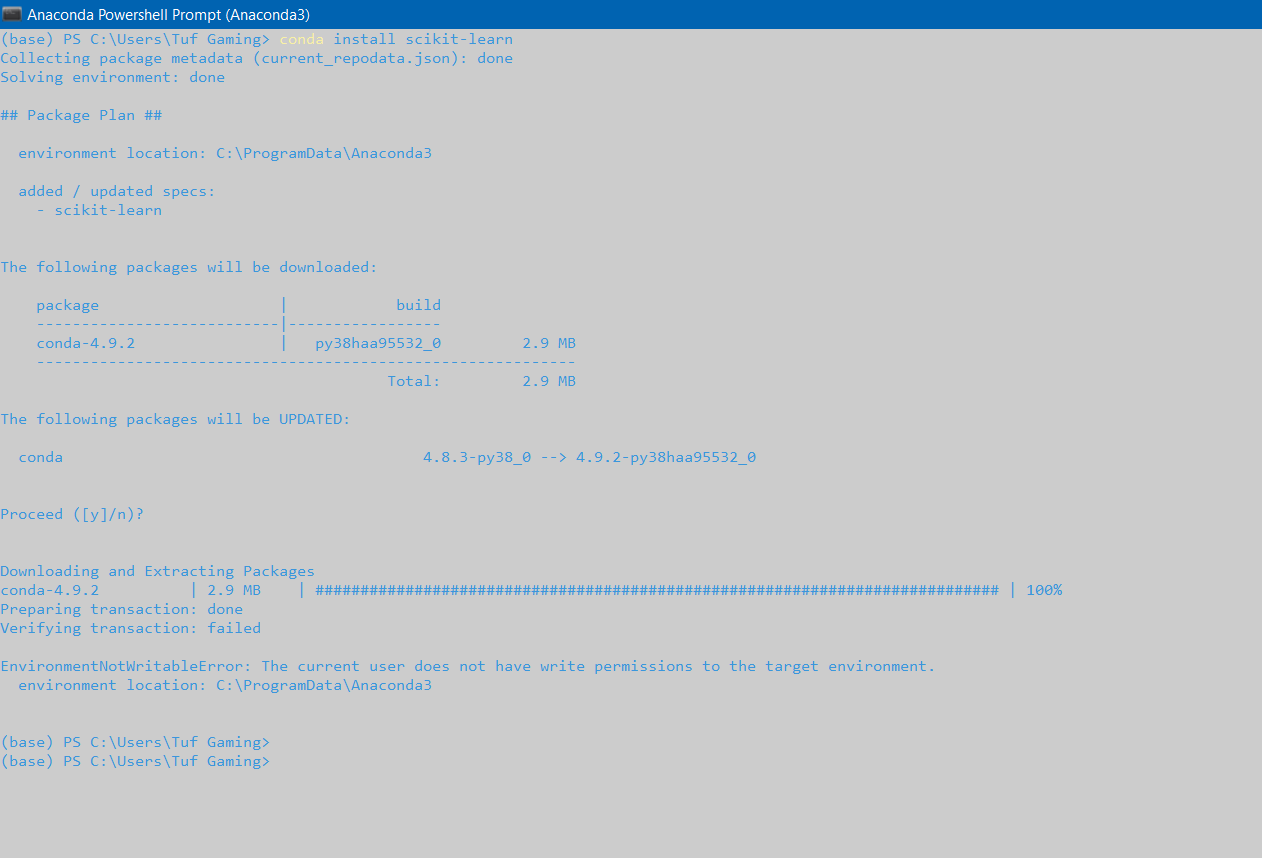
\includegraphics[width=10cm]{figures/1184053/chapter1/1.PNG}
		\centering
		\caption{Instalasi Package Scikit Learn}
	\end{figure}
	\begin{figure}[H]
		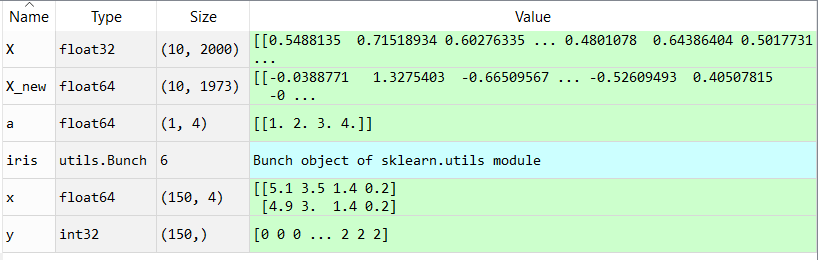
\includegraphics[width=10cm]{figures/1184053/chapter1/2.PNG}
		\centering
		\caption{Isi Variabel Explorer}
	\end{figure}
	\item Mencoba loading an example dataset
	\hfill\break
	\lstinputlisting[firstline=8, lastline=12]{src/1184053/chapter1/1184053.py}
	\item Mencoba Learning dan predicting
	\hfill\break
	\lstinputlisting[firstline=14, lastline=24]{src/1184053/chapter1/1184053.py}
	\item Mencoba Model Persistence
	\hfill\break
	\lstinputlisting[firstline=26, lastline=36]{src/1184053/chapter1/1184053.py}
	\item Mencoba Conventions
	\hfill\break
	\lstinputlisting[firstline=38, lastline=50]{src/1184053/chapter1/1184053.py}
\end{enumerate}
\subsection{Penanganan Error}
\begin{enumerate}
	\item ScreenShoot Error
	\begin{figure}[H]
		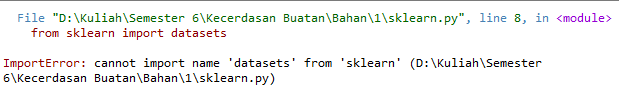
\includegraphics[width=10cm]{figures/1184053/chapter1/3.png}
		\centering
		\caption{Import Error}
	\end{figure}
	\begin{figure}[H]
		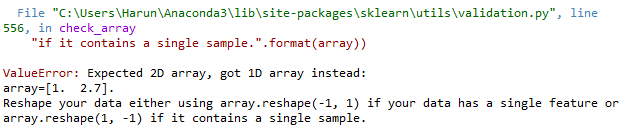
\includegraphics[width=10cm]{figures/1184053/chapter1/4.png}
		\centering
		\caption{Value Error}
	\end{figure}
	\item Tuliskan Kode Error dan Jenis Error
	\begin{itemize}
		\item Import Error
		\item Value Error
	\end{itemize}
	\item Cara Penangan Error
	\begin{itemize}
		\item Import Error
		\hfill\break
		Dengan Menginstall Library Yang Tidak Ditemukan
		\item Value Error
		\hfill\break
		Mengubah Bentuk Arraynya, Menjadi 1 Dimensi
	\end{itemize}
\end{enumerate}
	\subsection{Bukti Tidak Plagiat}
\begin{figure}[h]
	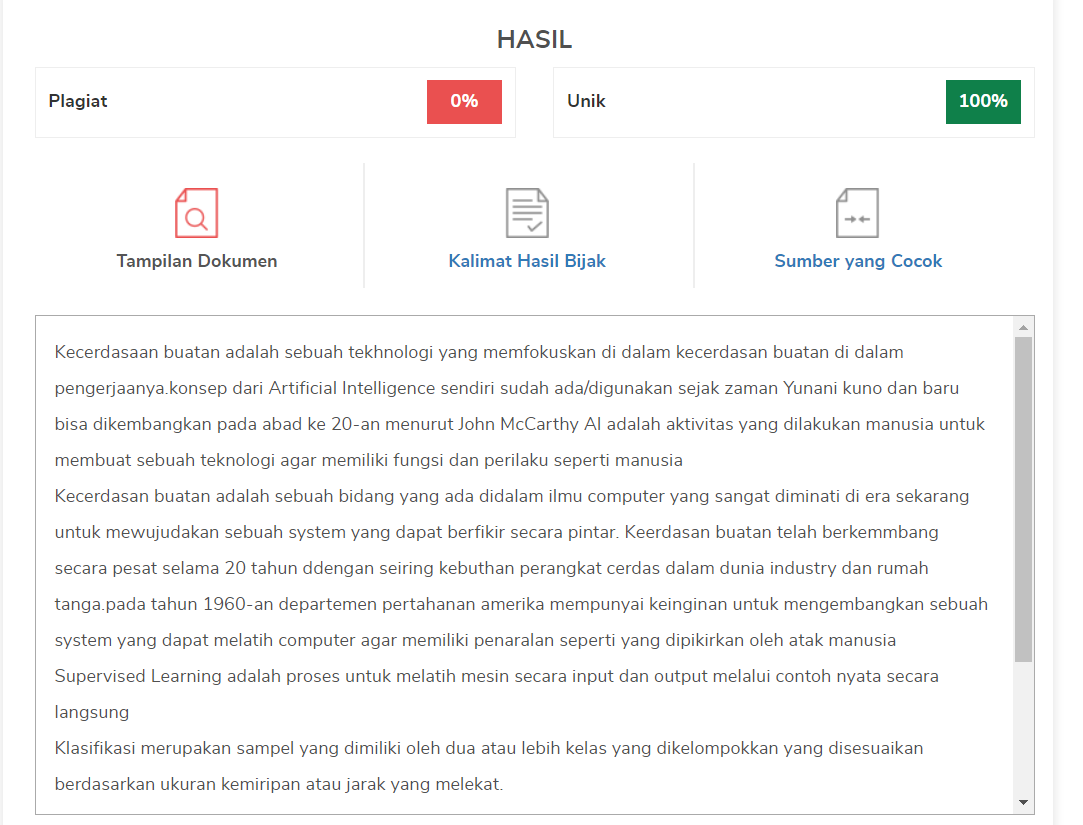
\includegraphics[width=10cm]{figures/1184053/chapter1/plagiat.png}
	\centering
	\caption{Bukti Tidak Melakukan Plagiat Chapter 1}
\end{figure}